    \hypertarget{unit-3.3-grovers-algorithm}{%
	\section{Jupyter Notebook Unit 3.3 : Grover's Algorithm and Amplitude Amplification}\label{unit-3.3-grovers-algorithm}}

\hypertarget{grover}{%
	\subsection*{Grover's search algorithm}\label{grover}}
    

The algorithm is often described as finding ``a needle in a haystack''.
Suppose we have a large search space of size \(N\), and one (or more) of
the elements is special. If a classical algorithm, in the worst case we
would need to look through all \(N\) elements to find our solution(s).
In a randomized algorithm, we would expect to find the solution in
\(\frac{N}{2}\), still \(O(N)\).

Grover can do this in about \(O(\sqrt{N})\) iterations.

\hypertarget{how-does-it-work}{%
\subsubsection*{How does it work}\label{how-does-it-work}}

We use a black-box function, or Oracle, that can quickly verify that an
input is a solution to some problem.

We can think of this as nudging, or jiggling, the quantum state in a way
that attracts it to the desired solution state.

The algorithm then has three steps:

\begin{enumerate}
\def\labelenumi{\arabic{enumi}.}
\item
  Start in complete ignorance (equal superposition). We setup a state
  that all possible answers are equally likely by applying the Hadamard
  gate to all n qubits.
\item
  Construct an Oracle gate to mark the correct state.
\item
  Amplify the correct answer by applying the \emph{Grover Diffusion
  Operator} to reflect the quantum state around the average amplitude.
  For each iteration, the amplitude (probability) of the correct answer
  increases, and the others decrease.
\end{enumerate}

When we measure the qubits at the end of these iterations, we will have,
with a high probability, the correct answer.

    As noted in \emph{Neilsen and Cheung}:

\begin{quote}
It seems as though the oracle already \emph{knows} the answer to the
search problem; what possible use could it be to have a quantum serach
algorithm based upon such oracle consultations?! The answer is that
there is a distinction between \emph{knowing} the solution to a search
problem, and being able to \emph{recognize} the solution; the crucial
point is that it is possible to do the latter without necessarily being
able to do the former.
\end{quote}

When looking for \(M\) solutions in a search space of size \(N\), the
sum over all non-solutions is the state:

\(|\alpha \rangle = \frac{1}{\sqrt{N-M}} \sum^{''}_{x}{|x\rangle}\).

The sum over x which are solutions is:

\(|\beta \rangle = \frac{1}{\sqrt{M}} \sum^{'}_{x}{|x\rangle}\).

These states are obviously orthogonal.

We can visualise the Grover operation, \(G\), as two rotations in a
2-dimension space, spanned by the starting vector
\(|\psi \rangle = \sqrt{\frac{N-M}{N}}|\alpha\rangle + \sqrt{\frac{M}{N}}|\beta\rangle\),
where \(|\psi\rangle\) is the uniform superposition of search space
solutions.

So the initial state is in the space spanned by \(|\alpha\rangle\) and
\(|\beta\rangle\)

\begin{figure}
	\centering
	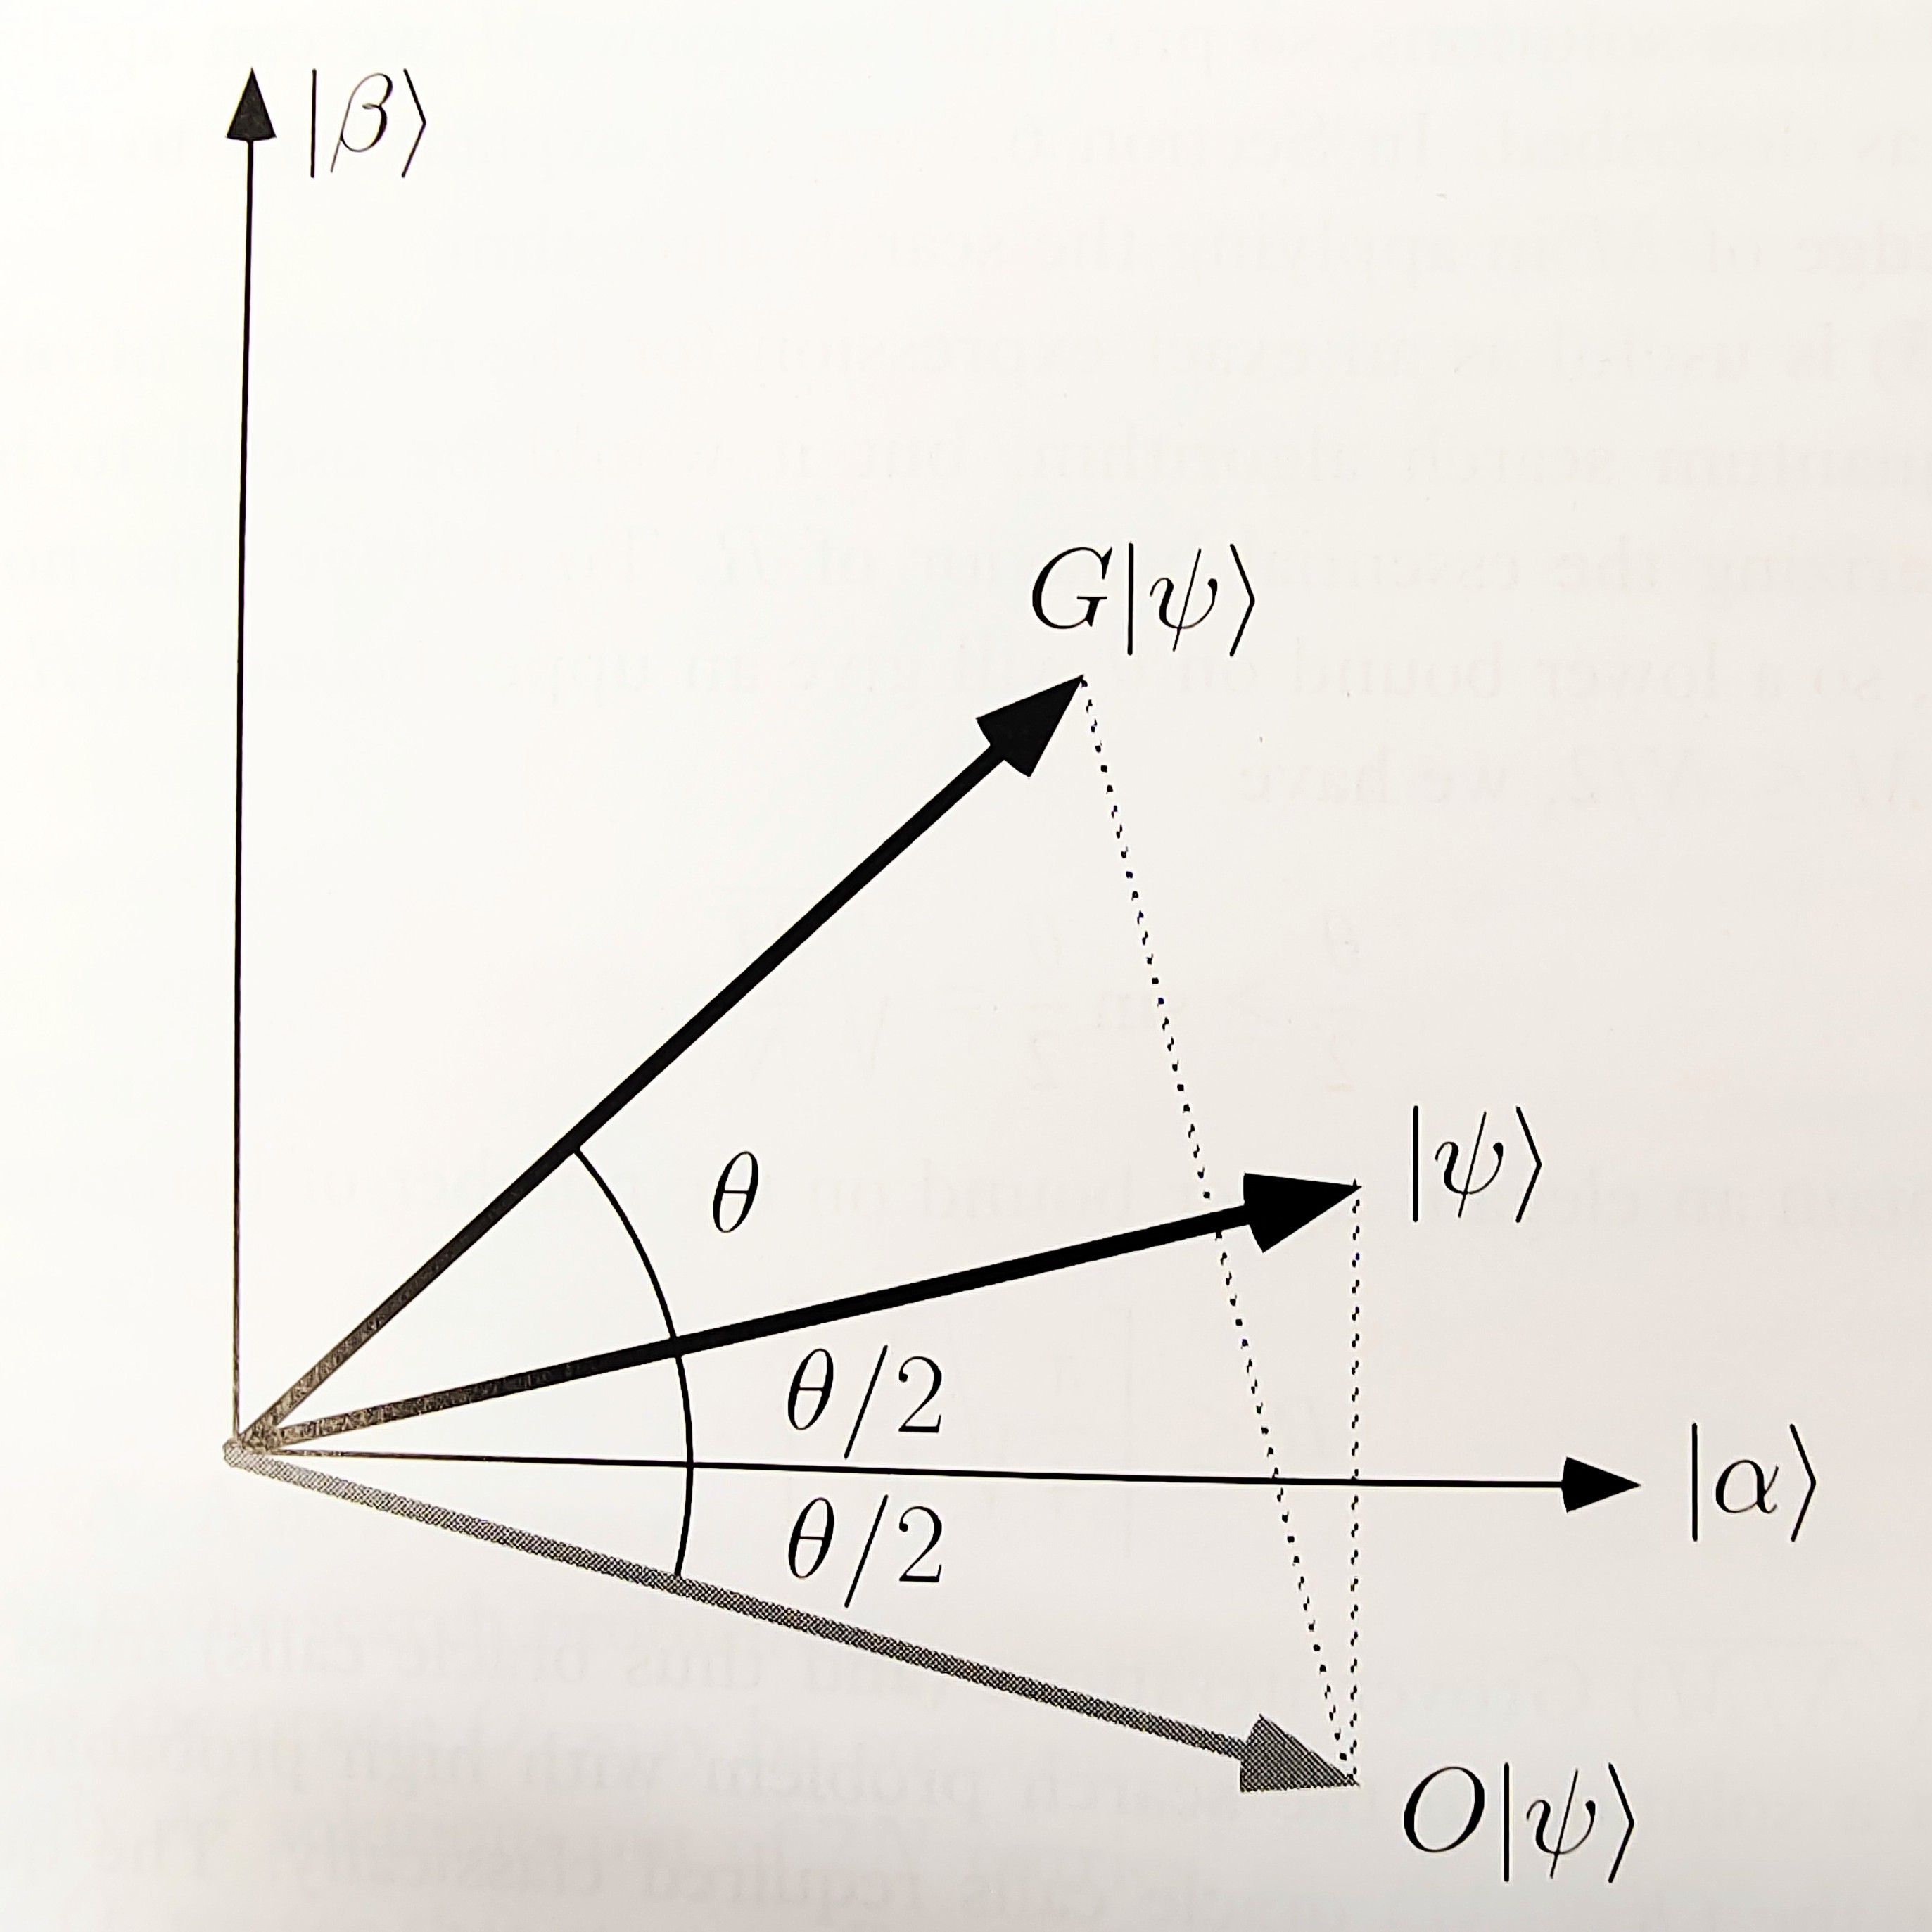
\includegraphics{figures/single_grover_iteration.jpg}
	\caption{Application Grover Oracle Operator(copyright Nielsen \& Chuang 2010)}
\end{figure}

The Grover operator applies the oracle operator \(O\) phase shift to
\(|\psi\rangle\), to mark the solution.\\
\(O|\psi\rangle\) is a reflection of the initial state vector
\(|\psi\rangle\) about the state \(|\alpha\rangle\).

The Grover algorithm then applies a \(2|\psi\rangle\langle\psi| - I\)
reflection about \(|\psi\rangle\).

The pair of reflections is guaranteed to leave the new state
\(G|\psi\rangle\) in the space spanned by \(|\alpha\rangle\) and
\(|\beta\rangle\).

    \hypertarget{qiskit-implementation}{%
\subsubsection*{QISKIT Implementation}\label{qiskit-implementation}}

In our set-up, using the QISKIT components, the Oracle marks the correct
solution by flipping the \emph{phase} of the correct state.\\
We will see that we do this by setting up a Unitary matrix operator,
with the phase flipped.

    \begin{tcolorbox}[breakable, size=fbox, boxrule=1pt, pad at break*=1mm,colback=cellbackground, colframe=cellborder]
\prompt{In}{incolor}{1}{\boxspacing}
\begin{Verbatim}[commandchars=\\\{\}]
\PY{k+kn}{import} \PY{n+nn}{numpy} \PY{k}{as} \PY{n+nn}{np}
\PY{k+kn}{from} \PY{n+nn}{qiskit} \PY{k+kn}{import} \PY{n}{QuantumCircuit}\PY{p}{,} \PY{n}{transpile}\PY{p}{,} \PY{n}{QuantumRegister}\PY{p}{,} \PY{n}{ClassicalRegister}
\PY{k+kn}{from} \PY{n+nn}{qiskit}\PY{n+nn}{.}\PY{n+nn}{visualization} \PY{k+kn}{import} \PY{n}{plot\PYZus{}histogram}
\PY{k+kn}{from} \PY{n+nn}{qiskit}\PY{n+nn}{.}\PY{n+nn}{circuit}\PY{n+nn}{.}\PY{n+nn}{library} \PY{k+kn}{import} \PY{n}{GroverOperator}
\PY{k+kn}{from} \PY{n+nn}{qiskit\PYZus{}aer} \PY{k+kn}{import} \PY{n}{AerSimulator}
\PY{k+kn}{import} \PY{n+nn}{matplotlib}\PY{n+nn}{.}\PY{n+nn}{pyplot} \PY{k}{as} \PY{n+nn}{plt}

\PY{c+c1}{\PYZsh{} Create oracle matrix}
\PY{n}{n} \PY{o}{=} \PY{l+m+mi}{4}
\PY{n}{solutions} \PY{o}{=} \PY{p}{[}\PY{l+m+mi}{3}\PY{p}{,} \PY{l+m+mi}{5}\PY{p}{]}
\PY{n}{size} \PY{o}{=} \PY{l+m+mi}{2} \PY{o}{*}\PY{o}{*} \PY{n}{n}
\PY{n}{oracle} \PY{o}{=} \PY{n}{np}\PY{o}{.}\PY{n}{eye}\PY{p}{(}\PY{n}{size}\PY{p}{)}
\PY{k}{for} \PY{n}{idx} \PY{o+ow}{in} \PY{n}{solutions}\PY{p}{:}
    \PY{n}{oracle}\PY{p}{[}\PY{n}{idx}\PY{p}{,} \PY{n}{idx}\PY{p}{]} \PY{o}{=} \PY{o}{\PYZhy{}}\PY{l+m+mi}{1}
\PY{n+nb}{print}\PY{p}{(}\PY{l+s+sa}{f}\PY{l+s+s2}{\PYZdq{}}\PY{l+s+s2}{With }\PY{l+s+si}{\PYZob{}}\PY{n}{n}\PY{l+s+si}{\PYZcb{}}\PY{l+s+s2}{ qubits, we have a hilbert space of size }\PY{l+s+si}{\PYZob{}}\PY{l+m+mi}{2}\PY{+w}{ }\PY{o}{*}\PY{o}{*}\PY{+w}{ }\PY{n}{n}\PY{l+s+si}{\PYZcb{}}\PY{l+s+s2}{\PYZdq{}}\PY{p}{)}
\PY{n+nb}{print}\PY{p}{(}\PY{n}{oracle}\PY{p}{)}

\PY{c+c1}{\PYZsh{} Convert to quantum circuit}
\PY{n}{oracle\PYZus{}circuit} \PY{o}{=} \PY{n}{QuantumCircuit}\PY{p}{(}\PY{n}{n}\PY{p}{)}
\PY{n}{oracle\PYZus{}circuit}\PY{o}{.}\PY{n}{unitary}\PY{p}{(}\PY{n}{oracle}\PY{p}{,} \PY{n+nb}{range}\PY{p}{(}\PY{n}{n}\PY{p}{)}\PY{p}{,} \PY{n}{label}\PY{o}{=}\PY{l+s+s2}{\PYZdq{}}\PY{l+s+s2}{Oracle}\PY{l+s+s2}{\PYZdq{}}\PY{p}{)}
\PY{n}{oracle\PYZus{}circuit}\PY{o}{.}\PY{n}{decompose}\PY{p}{(}\PY{p}{)}\PY{o}{.}\PY{n}{draw}\PY{p}{(}\PY{l+s+s2}{\PYZdq{}}\PY{l+s+s2}{mpl}\PY{l+s+s2}{\PYZdq{}}\PY{p}{)}
\end{Verbatim}
\end{tcolorbox}

    \begin{Verbatim}[commandchars=\\\{\}]
With 4 qubits, we have a hilbert space of size 16
[[ 1.  0.  0.  0.  0.  0.  0.  0.  0.  0.  0.  0.  0.  0.  0.  0.]
 [ 0.  1.  0.  0.  0.  0.  0.  0.  0.  0.  0.  0.  0.  0.  0.  0.]
 [ 0.  0.  1.  0.  0.  0.  0.  0.  0.  0.  0.  0.  0.  0.  0.  0.]
 [ 0.  0.  0. -1.  0.  0.  0.  0.  0.  0.  0.  0.  0.  0.  0.  0.]
 [ 0.  0.  0.  0.  1.  0.  0.  0.  0.  0.  0.  0.  0.  0.  0.  0.]
 [ 0.  0.  0.  0.  0. -1.  0.  0.  0.  0.  0.  0.  0.  0.  0.  0.]
 [ 0.  0.  0.  0.  0.  0.  1.  0.  0.  0.  0.  0.  0.  0.  0.  0.]
 [ 0.  0.  0.  0.  0.  0.  0.  1.  0.  0.  0.  0.  0.  0.  0.  0.]
 [ 0.  0.  0.  0.  0.  0.  0.  0.  1.  0.  0.  0.  0.  0.  0.  0.]
 [ 0.  0.  0.  0.  0.  0.  0.  0.  0.  1.  0.  0.  0.  0.  0.  0.]
 [ 0.  0.  0.  0.  0.  0.  0.  0.  0.  0.  1.  0.  0.  0.  0.  0.]
 [ 0.  0.  0.  0.  0.  0.  0.  0.  0.  0.  0.  1.  0.  0.  0.  0.]
 [ 0.  0.  0.  0.  0.  0.  0.  0.  0.  0.  0.  0.  1.  0.  0.  0.]
 [ 0.  0.  0.  0.  0.  0.  0.  0.  0.  0.  0.  0.  0.  1.  0.  0.]
 [ 0.  0.  0.  0.  0.  0.  0.  0.  0.  0.  0.  0.  0.  0.  1.  0.]
 [ 0.  0.  0.  0.  0.  0.  0.  0.  0.  0.  0.  0.  0.  0.  0.  1.]]
    \end{Verbatim}
 
            
\prompt{Out}{outcolor}{1}{}
    
    \begin{center}
    \adjustimage{max size={0.9\linewidth}{0.9\paperheight}}{figures/unit_3.3_grovers_algorithm_3_1.png}
    \end{center}
    { \hspace*{\fill} \\}
    

    \begin{tcolorbox}[breakable, size=fbox, boxrule=1pt, pad at break*=1mm,colback=cellbackground, colframe=cellborder]
\prompt{In}{incolor}{2}{\boxspacing}
\begin{Verbatim}[commandchars=\\\{\}]
\PY{c+c1}{\PYZsh{} Calculate optimal number of iterations}
\PY{n}{k} \PY{o}{=} \PY{n+nb}{max}\PY{p}{(}\PY{l+m+mi}{1}\PY{p}{,} \PY{n+nb}{int}\PY{p}{(}\PY{n}{np}\PY{o}{.}\PY{n}{floor}\PY{p}{(}\PY{p}{(}\PY{n}{np}\PY{o}{.}\PY{n}{pi} \PY{o}{/} \PY{l+m+mi}{4}\PY{p}{)} \PY{o}{*} \PY{n}{np}\PY{o}{.}\PY{n}{sqrt}\PY{p}{(}\PY{l+m+mi}{2} \PY{o}{*}\PY{o}{*} \PY{n}{n} \PY{o}{/} \PY{n+nb}{len}\PY{p}{(}\PY{n}{solutions}\PY{p}{)}\PY{p}{)}\PY{p}{)}\PY{p}{)}\PY{p}{,} \PY{l+m+mi}{0}\PY{p}{)}

\PY{c+c1}{\PYZsh{} Create quantum and classical registers}
\PY{n}{qn} \PY{o}{=} \PY{n}{QuantumRegister}\PY{p}{(}\PY{n}{n}\PY{p}{,} \PY{l+s+s1}{\PYZsq{}}\PY{l+s+s1}{qn}\PY{l+s+s1}{\PYZsq{}}\PY{p}{)}
\PY{n}{c} \PY{o}{=} \PY{n}{ClassicalRegister}\PY{p}{(}\PY{n}{n}\PY{p}{,} \PY{l+s+s1}{\PYZsq{}}\PY{l+s+s1}{c}\PY{l+s+s1}{\PYZsq{}}\PY{p}{)}
\PY{n}{qc} \PY{o}{=} \PY{n}{QuantumCircuit}\PY{p}{(}\PY{n}{qn}\PY{p}{,} \PY{n}{c}\PY{p}{)}

\PY{c+c1}{\PYZsh{} Initialize superposition}
\PY{n}{qc}\PY{o}{.}\PY{n}{h}\PY{p}{(}\PY{n}{qn}\PY{p}{)}
        
\PY{c+c1}{\PYZsh{} Create the grover operator to apply the reflections, and apply for k iterations}
\PY{n}{grover\PYZus{}operator} \PY{o}{=} \PY{n}{GroverOperator}\PY{p}{(}\PY{n}{oracle\PYZus{}circuit}\PY{p}{)}

\PY{k}{for} \PY{n}{\PYZus{}} \PY{o+ow}{in} \PY{n+nb}{range}\PY{p}{(}\PY{n}{k}\PY{p}{)}\PY{p}{:}
    \PY{n}{qc}\PY{o}{.}\PY{n}{append}\PY{p}{(}\PY{n}{grover\PYZus{}operator}\PY{p}{,} \PY{n}{qn}\PY{p}{)}

\PY{c+c1}{\PYZsh{} Measure results}
\PY{n}{qc}\PY{o}{.}\PY{n}{measure}\PY{p}{(}\PY{n}{qn}\PY{p}{,} \PY{n}{c}\PY{p}{)}
\PY{n}{qc}\PY{o}{.}\PY{n}{draw}\PY{p}{(}\PY{l+s+s2}{\PYZdq{}}\PY{l+s+s2}{mpl}\PY{l+s+s2}{\PYZdq{}}\PY{p}{)}
\end{Verbatim}
\end{tcolorbox}
 
            
\prompt{Out}{outcolor}{2}{}
    
    \begin{center}
    \adjustimage{max size={0.9\linewidth}{0.9\paperheight}}{figures/unit_3.3_grovers_algorithm_4_0.png}
    \end{center}
    { \hspace*{\fill} \\}
    

    \begin{tcolorbox}[breakable, size=fbox, boxrule=1pt, pad at break*=1mm,colback=cellbackground, colframe=cellborder]
\prompt{In}{incolor}{3}{\boxspacing}
\begin{Verbatim}[commandchars=\\\{\}]
\PY{n+nb}{print}\PY{p}{(}\PY{l+s+sa}{f}\PY{l+s+s2}{\PYZdq{}}\PY{l+s+s2}{Simple Grover}\PY{l+s+s2}{\PYZsq{}}\PY{l+s+s2}{s Algorithm Circuit}\PY{l+s+se}{\PYZbs{}n}\PY{l+s+s2}{\PYZdq{}}
      \PY{l+s+sa}{f}\PY{l+s+s2}{\PYZdq{}}\PY{l+s+s2}{Searching for }\PY{l+s+si}{\PYZob{}}\PY{n+nb}{len}\PY{p}{(}\PY{n}{solutions}\PY{p}{)}\PY{l+s+si}{\PYZcb{}}\PY{l+s+s2}{ solution}\PY{l+s+si}{\PYZob{}}\PY{l+s+s1}{\PYZsq{}}\PY{l+s+s1}{s}\PY{l+s+s1}{\PYZsq{}}\PY{+w}{ }\PY{k}{if}\PY{+w}{ }\PY{n+nb}{len}\PY{p}{(}\PY{n}{solutions}\PY{p}{)}\PY{o}{\PYZgt{}}\PY{l+m+mi}{1}\PY{+w}{ }\PY{k}{else}\PY{+w}{ }\PY{l+s+s1}{\PYZsq{}}\PY{l+s+s1}{\PYZsq{}}\PY{l+s+si}{\PYZcb{}}\PY{l+s+s2}{ }\PY{l+s+s2}{\PYZdq{}}
      \PY{l+s+sa}{f}\PY{l+s+s2}{\PYZdq{}}\PY{l+s+s2}{in }\PY{l+s+si}{\PYZob{}}\PY{l+m+mi}{2}\PY{o}{*}\PY{o}{*}\PY{n}{n}\PY{l+s+si}{\PYZcb{}}\PY{l+s+s2}{ states}\PY{l+s+se}{\PYZbs{}n}\PY{l+s+s2}{\PYZdq{}}
      \PY{l+s+sa}{f}\PY{l+s+s2}{\PYZdq{}}\PY{l+s+s2}{Number of iterations: }\PY{l+s+si}{\PYZob{}}\PY{n}{qc}\PY{o}{.}\PY{n}{count\PYZus{}ops}\PY{p}{(}\PY{p}{)}\PY{o}{.}\PY{n}{get}\PY{p}{(}\PY{l+s+s1}{\PYZsq{}}\PY{l+s+s1}{Q}\PY{l+s+s1}{\PYZsq{}}\PY{p}{,}\PY{+w}{ }\PY{l+m+mi}{0}\PY{p}{)}\PY{l+s+si}{\PYZcb{}}\PY{l+s+se}{\PYZbs{}n}\PY{l+s+s2}{\PYZdq{}}\PY{p}{)}

\PY{n+nb}{print}\PY{p}{(}\PY{l+s+sa}{f}\PY{l+s+s2}{\PYZdq{}}\PY{l+s+s2}{Circuit Statistics:}\PY{l+s+se}{\PYZbs{}n}\PY{l+s+s2}{\PYZdq{}}
      \PY{l+s+sa}{f}\PY{l+s+s2}{\PYZdq{}}\PY{l+s+s2}{Qubits: }\PY{l+s+si}{\PYZob{}}\PY{n}{n}\PY{l+s+si}{\PYZcb{}}\PY{l+s+se}{\PYZbs{}n}\PY{l+s+s2}{\PYZdq{}}
      \PY{l+s+sa}{f}\PY{l+s+s2}{\PYZdq{}}\PY{l+s+s2}{Gates: }\PY{l+s+si}{\PYZob{}}\PY{n+nb}{sum}\PY{p}{(}\PY{n}{qc}\PY{o}{.}\PY{n}{count\PYZus{}ops}\PY{p}{(}\PY{p}{)}\PY{o}{.}\PY{n}{values}\PY{p}{(}\PY{p}{)}\PY{p}{)}\PY{l+s+si}{\PYZcb{}}\PY{l+s+se}{\PYZbs{}n}\PY{l+s+s2}{\PYZdq{}}
      \PY{l+s+sa}{f}\PY{l+s+s2}{\PYZdq{}}\PY{l+s+s2}{Depth: }\PY{l+s+si}{\PYZob{}}\PY{n}{qc}\PY{o}{.}\PY{n}{depth}\PY{p}{(}\PY{p}{)}\PY{l+s+si}{\PYZcb{}}\PY{l+s+s2}{\PYZdq{}}\PY{p}{)}

\PY{c+c1}{\PYZsh{} Run simulation}
\PY{n}{simulator} \PY{o}{=} \PY{n}{AerSimulator}\PY{p}{(}\PY{p}{)}
\PY{n}{qc\PYZus{}t} \PY{o}{=} \PY{n}{transpile}\PY{p}{(}\PY{n}{qc}\PY{p}{,} \PY{n}{simulator}\PY{p}{)}
\PY{n}{result} \PY{o}{=} \PY{n}{simulator}\PY{o}{.}\PY{n}{run}\PY{p}{(}\PY{n}{qc\PYZus{}t}\PY{p}{,} \PY{n}{shots}\PY{o}{=}\PY{l+m+mi}{300}\PY{p}{)}\PY{o}{.}\PY{n}{result}\PY{p}{(}\PY{p}{)}
\PY{n}{counts} \PY{o}{=} \PY{n}{result}\PY{o}{.}\PY{n}{get\PYZus{}counts}\PY{p}{(}\PY{p}{)}

\PY{n}{plot\PYZus{}histogram}\PY{p}{(}\PY{n}{counts}\PY{p}{)}
\end{Verbatim}
\end{tcolorbox}

    \begin{Verbatim}[commandchars=\\\{\}]
Simple Grover's Algorithm Circuit
Searching for 2 solutions in 16 states
Number of iterations: 2

Circuit Statistics:
Qubits: 4
Gates: 10
Depth: 4
    \end{Verbatim}
 
            
\prompt{Out}{outcolor}{3}{}
    
    \begin{center}
    \adjustimage{max size={0.9\linewidth}{0.9\paperheight}}{figures/unit_3.3_grovers_algorithm_5_1.png}
    \end{center}
    { \hspace*{\fill} \\}
    

    \hypertarget{running-grovers-algorithm}{%
\subsection*{Running Grover's
algorithm}\label{running-grovers-algorithm}}

This is the code from the IBM tutorial
\href{https://qiskit-community.github.io/qiskit-algorithms/tutorials/06_grover.html}{IBM
QISKIT Grover notebook source}

Specify an oracle for the circuit of Grover's algorithm.

    \begin{tcolorbox}[breakable, size=fbox, boxrule=1pt, pad at break*=1mm,colback=cellbackground, colframe=cellborder]
\prompt{In}{incolor}{4}{\boxspacing}
\begin{Verbatim}[commandchars=\\\{\}]
\PY{k+kn}{from} \PY{n+nn}{qiskit} \PY{k+kn}{import} \PY{n}{QuantumCircuit}
\PY{k+kn}{from} \PY{n+nn}{qiskit\PYZus{}algorithms} \PY{k+kn}{import} \PY{n}{AmplificationProblem}

\PY{c+c1}{\PYZsh{} the state we desire to find is \PYZsq{}11\PYZsq{}}
\PY{n}{good\PYZus{}state} \PY{o}{=} \PY{p}{[}\PY{l+s+s2}{\PYZdq{}}\PY{l+s+s2}{11}\PY{l+s+s2}{\PYZdq{}}\PY{p}{]}

\PY{c+c1}{\PYZsh{} specify the oracle that marks the state \PYZsq{}11\PYZsq{} as a good solution}
\PY{n}{oracle} \PY{o}{=} \PY{n}{QuantumCircuit}\PY{p}{(}\PY{l+m+mi}{2}\PY{p}{)}
\PY{n}{oracle}\PY{o}{.}\PY{n}{cz}\PY{p}{(}\PY{l+m+mi}{0}\PY{p}{,} \PY{l+m+mi}{1}\PY{p}{)}

\PY{c+c1}{\PYZsh{} define Grover\PYZsq{}s algorithm}
\PY{n}{problem} \PY{o}{=} \PY{n}{AmplificationProblem}\PY{p}{(}\PY{n}{oracle}\PY{p}{,} \PY{n}{is\PYZus{}good\PYZus{}state}\PY{o}{=}\PY{n}{good\PYZus{}state}\PY{p}{)}

\PY{c+c1}{\PYZsh{} now we can have a look at the Grover operator that is used in running the algorithm}
\PY{c+c1}{\PYZsh{} (Algorithm circuits are wrapped in a gate to appear in composition as a block}
\PY{c+c1}{\PYZsh{} so we have to decompose() the op to see it expanded into its component gates.)}
\PY{n}{problem}\PY{o}{.}\PY{n}{grover\PYZus{}operator}\PY{o}{.}\PY{n}{decompose}\PY{p}{(}\PY{p}{)}\PY{o}{.}\PY{n}{draw}\PY{p}{(}\PY{n}{output}\PY{o}{=}\PY{l+s+s2}{\PYZdq{}}\PY{l+s+s2}{mpl}\PY{l+s+s2}{\PYZdq{}}\PY{p}{)}
\end{Verbatim}
\end{tcolorbox}
 
            
\prompt{Out}{outcolor}{4}{}
    
    \begin{center}
    \adjustimage{max size={0.9\linewidth}{0.9\paperheight}}{figures/unit_3.3_grovers_algorithm_7_0.png}
    \end{center}
    { \hspace*{\fill} \\}
    

    Specify a backend to execute the circuits. Notice that we find a ``good
state'' in the `top\_measurement'.

    \begin{tcolorbox}[breakable, size=fbox, boxrule=1pt, pad at break*=1mm,colback=cellbackground, colframe=cellborder]
\prompt{In}{incolor}{5}{\boxspacing}
\begin{Verbatim}[commandchars=\\\{\}]
\PY{k+kn}{from} \PY{n+nn}{qiskit\PYZus{}algorithms} \PY{k+kn}{import} \PY{n}{Grover}
\PY{k+kn}{from} \PY{n+nn}{qiskit}\PY{n+nn}{.}\PY{n+nn}{primitives} \PY{k+kn}{import} \PY{n}{Sampler}

\PY{n}{grover} \PY{o}{=} \PY{n}{Grover}\PY{p}{(}\PY{n}{sampler}\PY{o}{=}\PY{n}{Sampler}\PY{p}{(}\PY{p}{)}\PY{p}{)}
\PY{n}{result} \PY{o}{=} \PY{n}{grover}\PY{o}{.}\PY{n}{amplify}\PY{p}{(}\PY{n}{problem}\PY{p}{)}
\PY{n+nb}{print}\PY{p}{(}\PY{l+s+s2}{\PYZdq{}}\PY{l+s+s2}{Result type:}\PY{l+s+s2}{\PYZdq{}}\PY{p}{,} \PY{n+nb}{type}\PY{p}{(}\PY{n}{result}\PY{p}{)}\PY{p}{)}
\PY{n+nb}{print}\PY{p}{(}\PY{p}{)}
\PY{n+nb}{print}\PY{p}{(}\PY{l+s+s2}{\PYZdq{}}\PY{l+s+s2}{Success!}\PY{l+s+s2}{\PYZdq{}} \PY{k}{if} \PY{n}{result}\PY{o}{.}\PY{n}{oracle\PYZus{}evaluation} \PY{k}{else} \PY{l+s+s2}{\PYZdq{}}\PY{l+s+s2}{Failure!}\PY{l+s+s2}{\PYZdq{}}\PY{p}{)}
\PY{n+nb}{print}\PY{p}{(}\PY{l+s+s2}{\PYZdq{}}\PY{l+s+s2}{Top measurement:}\PY{l+s+s2}{\PYZdq{}}\PY{p}{,} \PY{n}{result}\PY{o}{.}\PY{n}{top\PYZus{}measurement}\PY{p}{)}
\end{Verbatim}
\end{tcolorbox}

    \begin{Verbatim}[commandchars=\\\{\}]
Result type: <class
'qiskit\_algorithms.amplitude\_amplifiers.grover.GroverResult'>

Success!
Top measurement: 11
    \end{Verbatim}

    \begin{Verbatim}[commandchars=\\\{\}]
/tmp/ipykernel\_292492/4134062562.py:4: DeprecationWarning: The class
``qiskit.primitives.sampler.Sampler`` is deprecated as of qiskit 1.2. It will be
removed no earlier than 3 months after the release date. All implementations of
the `BaseSamplerV1` interface have been deprecated in favor of their V2
counterparts. The V2 alternative for the `Sampler` class is
`StatevectorSampler`.
  grover = Grover(sampler=Sampler())
    \end{Verbatim}

    We can use different QISKIT components as an Oracle. Here is the same
example, but using the \texttt{StateVector} instead.

    \begin{tcolorbox}[breakable, size=fbox, boxrule=1pt, pad at break*=1mm,colback=cellbackground, colframe=cellborder]
\prompt{In}{incolor}{6}{\boxspacing}
\begin{Verbatim}[commandchars=\\\{\}]
\PY{k+kn}{from} \PY{n+nn}{qiskit}\PY{n+nn}{.}\PY{n+nn}{quantum\PYZus{}info} \PY{k+kn}{import} \PY{n}{Statevector}

\PY{n}{oracle} \PY{o}{=} \PY{n}{Statevector}\PY{o}{.}\PY{n}{from\PYZus{}label}\PY{p}{(}\PY{l+s+s2}{\PYZdq{}}\PY{l+s+s2}{11}\PY{l+s+s2}{\PYZdq{}}\PY{p}{)}
\PY{n}{problem} \PY{o}{=} \PY{n}{AmplificationProblem}\PY{p}{(}\PY{n}{oracle}\PY{p}{,} \PY{n}{is\PYZus{}good\PYZus{}state}\PY{o}{=}\PY{p}{[}\PY{l+s+s2}{\PYZdq{}}\PY{l+s+s2}{11}\PY{l+s+s2}{\PYZdq{}}\PY{p}{]}\PY{p}{)}

\PY{n}{grover} \PY{o}{=} \PY{n}{Grover}\PY{p}{(}\PY{n}{sampler}\PY{o}{=}\PY{n}{Sampler}\PY{p}{(}\PY{p}{)}\PY{p}{)}
\PY{n}{result} \PY{o}{=} \PY{n}{grover}\PY{o}{.}\PY{n}{amplify}\PY{p}{(}\PY{n}{problem}\PY{p}{)}
\PY{n+nb}{print}\PY{p}{(}\PY{l+s+s2}{\PYZdq{}}\PY{l+s+s2}{Result type:}\PY{l+s+s2}{\PYZdq{}}\PY{p}{,} \PY{n+nb}{type}\PY{p}{(}\PY{n}{result}\PY{p}{)}\PY{p}{)}
\PY{n+nb}{print}\PY{p}{(}\PY{p}{)}
\PY{n+nb}{print}\PY{p}{(}\PY{l+s+s2}{\PYZdq{}}\PY{l+s+s2}{Success!}\PY{l+s+s2}{\PYZdq{}} \PY{k}{if} \PY{n}{result}\PY{o}{.}\PY{n}{oracle\PYZus{}evaluation} \PY{k}{else} \PY{l+s+s2}{\PYZdq{}}\PY{l+s+s2}{Failure!}\PY{l+s+s2}{\PYZdq{}}\PY{p}{)}
\PY{n+nb}{print}\PY{p}{(}\PY{l+s+s2}{\PYZdq{}}\PY{l+s+s2}{Top measurement:}\PY{l+s+s2}{\PYZdq{}}\PY{p}{,} \PY{n}{result}\PY{o}{.}\PY{n}{top\PYZus{}measurement}\PY{p}{)}
\end{Verbatim}
\end{tcolorbox}

    \begin{Verbatim}[commandchars=\\\{\}]
Result type: <class
'qiskit\_algorithms.amplitude\_amplifiers.grover.GroverResult'>

Success!
Top measurement: 11
    \end{Verbatim}

    \begin{Verbatim}[commandchars=\\\{\}]
/tmp/ipykernel\_292492/1906973721.py:6: DeprecationWarning: The class
``qiskit.primitives.sampler.Sampler`` is deprecated as of qiskit 1.2. It will be
removed no earlier than 3 months after the release date. All implementations of
the `BaseSamplerV1` interface have been deprecated in favor of their V2
counterparts. The V2 alternative for the `Sampler` class is
`StatevectorSampler`.
  grover = Grover(sampler=Sampler())
    \end{Verbatim}

    Internally, the statevector is mapped to a quantum circuit:

    \begin{tcolorbox}[breakable, size=fbox, boxrule=1pt, pad at break*=1mm,colback=cellbackground, colframe=cellborder]
\prompt{In}{incolor}{7}{\boxspacing}
\begin{Verbatim}[commandchars=\\\{\}]
\PY{n}{problem}\PY{o}{.}\PY{n}{grover\PYZus{}operator}\PY{o}{.}\PY{n}{oracle}\PY{o}{.}\PY{n}{decompose}\PY{p}{(}\PY{p}{)}\PY{o}{.}\PY{n}{draw}\PY{p}{(}\PY{n}{output}\PY{o}{=}\PY{l+s+s2}{\PYZdq{}}\PY{l+s+s2}{mpl}\PY{l+s+s2}{\PYZdq{}}\PY{p}{)}
\end{Verbatim}
\end{tcolorbox}
 
            
\prompt{Out}{outcolor}{7}{}
    
    \begin{center}
    \adjustimage{max size={0.9\linewidth}{0.9\paperheight}}{figures/unit_3.3_grovers_algorithm_13_0.png}
    \end{center}
    { \hspace*{\fill} \\}
    

    Qiskit allows for an easy construction of more complex oracles.\\
\texttt{PhaseOracle} is used for parsing logical expressions such as
`\textasciitilde a \textbar{} b', and is useful for solving 3-SAT
problems.

Here we use the \texttt{PhaseOracle} for the simple example of finding
the state \(|11>\), which corresponds to `a \& b'

It does this by implementing a phase flip when the state is \(|11>\).

    \begin{tcolorbox}[breakable, size=fbox, boxrule=1pt, pad at break*=1mm,colback=cellbackground, colframe=cellborder]
\prompt{In}{incolor}{8}{\boxspacing}
\begin{Verbatim}[commandchars=\\\{\}]
\PY{k+kn}{from} \PY{n+nn}{qiskit}\PY{n+nn}{.}\PY{n+nn}{circuit}\PY{n+nn}{.}\PY{n+nn}{library}\PY{n+nn}{.}\PY{n+nn}{phase\PYZus{}oracle} \PY{k+kn}{import} \PY{n}{PhaseOracle}
\PY{k+kn}{from} \PY{n+nn}{qiskit}\PY{n+nn}{.}\PY{n+nn}{exceptions} \PY{k+kn}{import} \PY{n}{MissingOptionalLibraryError}

\PY{c+c1}{\PYZsh{} `Oracle` (`PhaseOracle`) as the `oracle` argument}
\PY{n}{expression} \PY{o}{=} \PY{l+s+s2}{\PYZdq{}}\PY{l+s+s2}{(a \PYZam{} b)}\PY{l+s+s2}{\PYZdq{}}
\PY{k}{try}\PY{p}{:}
    \PY{n}{oracle} \PY{o}{=} \PY{n}{PhaseOracle}\PY{p}{(}\PY{n}{expression}\PY{p}{)}
    \PY{n}{problem} \PY{o}{=} \PY{n}{AmplificationProblem}\PY{p}{(}\PY{n}{oracle}\PY{p}{)}
    \PY{n}{display}\PY{p}{(}\PY{n}{problem}\PY{o}{.}\PY{n}{grover\PYZus{}operator}\PY{o}{.}\PY{n}{oracle}\PY{o}{.}\PY{n}{decompose}\PY{p}{(}\PY{p}{)}\PY{o}{.}\PY{n}{draw}\PY{p}{(}\PY{n}{output}\PY{o}{=}\PY{l+s+s2}{\PYZdq{}}\PY{l+s+s2}{mpl}\PY{l+s+s2}{\PYZdq{}}\PY{p}{)}\PY{p}{)}
\PY{k}{except} \PY{n}{MissingOptionalLibraryError} \PY{k}{as} \PY{n}{ex}\PY{p}{:}
    \PY{n+nb}{print}\PY{p}{(}\PY{n}{ex}\PY{p}{)}
\end{Verbatim}
\end{tcolorbox}

    \begin{center}
    \adjustimage{max size={0.9\linewidth}{0.9\paperheight}}{figures/unit_3.3_grovers_algorithm_15_0.png}
    \end{center}
    { \hspace*{\fill} \\}
    
    \hypertarget{amplitude-amplification}{%
\subsubsection*{Amplitude Amplification}\label{amplitude-amplification}}

Grover's algorithm uses Hadamard gates to create the uniform
superposition of all the states at the beginning of the Grover operator
. If some information on the good states is available, it might be
useful to not start in a uniform superposition but only initialize
specific states. This, generalized, version of Grover's algorithm is
referred to Amplitude Amplification.

    \begin{tcolorbox}[breakable, size=fbox, boxrule=1pt, pad at break*=1mm,colback=cellbackground, colframe=cellborder]
\prompt{In}{incolor}{9}{\boxspacing}
\begin{Verbatim}[commandchars=\\\{\}]
\PY{k+kn}{import} \PY{n+nn}{numpy} \PY{k}{as} \PY{n+nn}{np}

\PY{c+c1}{\PYZsh{} Specifying `state\PYZus{}preparation`}
\PY{c+c1}{\PYZsh{} to prepare a superposition of |01\PYZgt{}, |10\PYZgt{}, and |11\PYZgt{}}
\PY{n}{oracle} \PY{o}{=} \PY{n}{QuantumCircuit}\PY{p}{(}\PY{l+m+mi}{3}\PY{p}{)}
\PY{n}{oracle}\PY{o}{.}\PY{n}{ccz}\PY{p}{(}\PY{l+m+mi}{0}\PY{p}{,} \PY{l+m+mi}{1}\PY{p}{,} \PY{l+m+mi}{2}\PY{p}{)}

\PY{n}{theta} \PY{o}{=} \PY{l+m+mi}{2} \PY{o}{*} \PY{n}{np}\PY{o}{.}\PY{n}{arccos}\PY{p}{(}\PY{l+m+mi}{1} \PY{o}{/} \PY{n}{np}\PY{o}{.}\PY{n}{sqrt}\PY{p}{(}\PY{l+m+mi}{3}\PY{p}{)}\PY{p}{)}
\PY{n}{state\PYZus{}preparation} \PY{o}{=} \PY{n}{QuantumCircuit}\PY{p}{(}\PY{l+m+mi}{3}\PY{p}{)}
\PY{n}{state\PYZus{}preparation}\PY{o}{.}\PY{n}{ry}\PY{p}{(}\PY{n}{theta}\PY{p}{,} \PY{l+m+mi}{0}\PY{p}{)}          \PY{c+c1}{\PYZsh{} Single\PYZhy{}qubit rotation about the Y axis.}
\PY{n}{state\PYZus{}preparation}\PY{o}{.}\PY{n}{ch}\PY{p}{(}\PY{l+m+mi}{0}\PY{p}{,} \PY{l+m+mi}{1}\PY{p}{)}              \PY{c+c1}{\PYZsh{} Applies a Hadamard on the target qubit if the control is in the ∣1⟩ state.}
\PY{n}{state\PYZus{}preparation}\PY{o}{.}\PY{n}{x}\PY{p}{(}\PY{l+m+mi}{1}\PY{p}{)}
\PY{n}{state\PYZus{}preparation}\PY{o}{.}\PY{n}{h}\PY{p}{(}\PY{l+m+mi}{2}\PY{p}{)}

\PY{c+c1}{\PYZsh{} we only care about the first two bits being in state 1, thus add both possibilities for the last qubit}
\PY{n}{problem} \PY{o}{=} \PY{n}{AmplificationProblem}\PY{p}{(}
    \PY{n}{oracle}\PY{p}{,} \PY{n}{state\PYZus{}preparation}\PY{o}{=}\PY{n}{state\PYZus{}preparation}\PY{p}{,} \PY{n}{is\PYZus{}good\PYZus{}state}\PY{o}{=}\PY{p}{[}\PY{l+s+s2}{\PYZdq{}}\PY{l+s+s2}{110}\PY{l+s+s2}{\PYZdq{}}\PY{p}{,} \PY{l+s+s2}{\PYZdq{}}\PY{l+s+s2}{111}\PY{l+s+s2}{\PYZdq{}}\PY{p}{]}
\PY{p}{)}

\PY{c+c1}{\PYZsh{} state\PYZus{}preparation}
\PY{n+nb}{print}\PY{p}{(}\PY{l+s+s2}{\PYZdq{}}\PY{l+s+s2}{state preparation circuit:}\PY{l+s+s2}{\PYZdq{}}\PY{p}{)}
\PY{n}{problem}\PY{o}{.}\PY{n}{grover\PYZus{}operator}\PY{o}{.}\PY{n}{state\PYZus{}preparation}\PY{o}{.}\PY{n}{draw}\PY{p}{(}\PY{n}{output}\PY{o}{=}\PY{l+s+s2}{\PYZdq{}}\PY{l+s+s2}{mpl}\PY{l+s+s2}{\PYZdq{}}\PY{p}{)}
\end{Verbatim}
\end{tcolorbox}

    \begin{Verbatim}[commandchars=\\\{\}]
state preparation circuit:
    \end{Verbatim}
 
            
\prompt{Out}{outcolor}{9}{}
    
    \begin{center}
    \adjustimage{max size={0.9\linewidth}{0.9\paperheight}}{figures/unit_3.3_grovers_algorithm_17_1.png}
    \end{center}
    { \hspace*{\fill} \\}
    

    \begin{tcolorbox}[breakable, size=fbox, boxrule=1pt, pad at break*=1mm,colback=cellbackground, colframe=cellborder]
\prompt{In}{incolor}{10}{\boxspacing}
\begin{Verbatim}[commandchars=\\\{\}]
\PY{k+kn}{from} \PY{n+nn}{qiskit}\PY{n+nn}{.}\PY{n+nn}{visualization} \PY{k+kn}{import} \PY{n}{plot\PYZus{}bloch\PYZus{}multivector}
\PY{n}{state} \PY{o}{=} \PY{n}{Statevector}\PY{p}{(}\PY{n}{state\PYZus{}preparation}\PY{p}{)}
\PY{n}{plot\PYZus{}bloch\PYZus{}multivector}\PY{p}{(}\PY{n}{state}\PY{p}{)}
\end{Verbatim}
\end{tcolorbox}
 
            
\prompt{Out}{outcolor}{10}{}
    
    \begin{center}
    \adjustimage{max size={0.9\linewidth}{0.9\paperheight}}{figures/unit_3.3_grovers_algorithm_18_0.png}
    \end{center}
    { \hspace*{\fill} \\}
    

    \begin{tcolorbox}[breakable, size=fbox, boxrule=1pt, pad at break*=1mm,colback=cellbackground, colframe=cellborder]
\prompt{In}{incolor}{11}{\boxspacing}
\begin{Verbatim}[commandchars=\\\{\}]
\PY{n}{grover} \PY{o}{=} \PY{n}{Grover}\PY{p}{(}\PY{n}{sampler}\PY{o}{=}\PY{n}{Sampler}\PY{p}{(}\PY{p}{)}\PY{p}{)}
\PY{n}{result} \PY{o}{=} \PY{n}{grover}\PY{o}{.}\PY{n}{amplify}\PY{p}{(}\PY{n}{problem}\PY{p}{)}
\PY{n+nb}{print}\PY{p}{(}\PY{l+s+s2}{\PYZdq{}}\PY{l+s+s2}{Success!}\PY{l+s+s2}{\PYZdq{}} \PY{k}{if} \PY{n}{result}\PY{o}{.}\PY{n}{oracle\PYZus{}evaluation} \PY{k}{else} \PY{l+s+s2}{\PYZdq{}}\PY{l+s+s2}{Failure!}\PY{l+s+s2}{\PYZdq{}}\PY{p}{)}
\PY{n+nb}{print}\PY{p}{(}\PY{l+s+s2}{\PYZdq{}}\PY{l+s+s2}{Top measurement:}\PY{l+s+s2}{\PYZdq{}}\PY{p}{,} \PY{n}{result}\PY{o}{.}\PY{n}{top\PYZus{}measurement}\PY{p}{)}
\end{Verbatim}
\end{tcolorbox}

    \begin{Verbatim}[commandchars=\\\{\}]
Success!
Top measurement: 111
    \end{Verbatim}

    \begin{Verbatim}[commandchars=\\\{\}]
/tmp/ipykernel\_292492/336064450.py:1: DeprecationWarning: The class
``qiskit.primitives.sampler.Sampler`` is deprecated as of qiskit 1.2. It will be
removed no earlier than 3 months after the release date. All implementations of
the `BaseSamplerV1` interface have been deprecated in favor of their V2
counterparts. The V2 alternative for the `Sampler` class is
`StatevectorSampler`.
  grover = Grover(sampler=Sampler())
    \end{Verbatim}

    \hypertarget{flexibilty}{%
\paragraph{Flexibilty}\label{flexibilty}}

As we saw at the top of the notebook, it is also possible to specify the
entire Grover operator by setting the grover\_operator argument.

    \begin{tcolorbox}[breakable, size=fbox, boxrule=1pt, pad at break*=1mm,colback=cellbackground, colframe=cellborder]
\prompt{In}{incolor}{12}{\boxspacing}
\begin{Verbatim}[commandchars=\\\{\}]
\PY{n}{oracle} \PY{o}{=} \PY{n}{QuantumCircuit}\PY{p}{(}\PY{l+m+mi}{5}\PY{p}{)}
\PY{n}{oracle}\PY{o}{.}\PY{n}{ccz}\PY{p}{(}\PY{l+m+mi}{0}\PY{p}{,} \PY{l+m+mi}{1}\PY{p}{,} \PY{l+m+mi}{2}\PY{p}{)}             \PY{c+c1}{\PYZsh{} flips the phase of the target qubit if the control qubits are in the ∣11⟩ state.}
\PY{n}{oracle}\PY{o}{.}\PY{n}{draw}\PY{p}{(}\PY{n}{output}\PY{o}{=}\PY{l+s+s2}{\PYZdq{}}\PY{l+s+s2}{mpl}\PY{l+s+s2}{\PYZdq{}}\PY{p}{)}
\end{Verbatim}
\end{tcolorbox}
 
            
\prompt{Out}{outcolor}{12}{}
    
    \begin{center}
    \adjustimage{max size={0.9\linewidth}{0.9\paperheight}}{figures/unit_3.3_grovers_algorithm_21_0.png}
    \end{center}
    { \hspace*{\fill} \\}
    

    \begin{tcolorbox}[breakable, size=fbox, boxrule=1pt, pad at break*=1mm,colback=cellbackground, colframe=cellborder]
\prompt{In}{incolor}{13}{\boxspacing}
\begin{Verbatim}[commandchars=\\\{\}]
\PY{k+kn}{from} \PY{n+nn}{qiskit}\PY{n+nn}{.}\PY{n+nn}{circuit}\PY{n+nn}{.}\PY{n+nn}{library} \PY{k+kn}{import} \PY{n}{GroverOperator}

\PY{n}{grover\PYZus{}op} \PY{o}{=} \PY{n}{GroverOperator}\PY{p}{(}\PY{n}{oracle}\PY{p}{,} \PY{n}{insert\PYZus{}barriers}\PY{o}{=}\PY{k+kc}{True}\PY{p}{)}
\PY{n}{grover\PYZus{}op}\PY{o}{.}\PY{n}{decompose}\PY{p}{(}\PY{p}{)}\PY{o}{.}\PY{n}{draw}\PY{p}{(}\PY{n}{output}\PY{o}{=}\PY{l+s+s2}{\PYZdq{}}\PY{l+s+s2}{mpl}\PY{l+s+s2}{\PYZdq{}}\PY{p}{)}
\end{Verbatim}
\end{tcolorbox}
 
            
\prompt{Out}{outcolor}{13}{}
    
    \begin{center}
    \adjustimage{max size={0.9\linewidth}{0.9\paperheight}}{figures/unit_3.3_grovers_algorithm_22_0.png}
    \end{center}
    { \hspace*{\fill} \\}
    

    But we know that we only need to consider the first three:

    \begin{tcolorbox}[breakable, size=fbox, boxrule=1pt, pad at break*=1mm,colback=cellbackground, colframe=cellborder]
\prompt{In}{incolor}{14}{\boxspacing}
\begin{Verbatim}[commandchars=\\\{\}]
\PY{n}{grover\PYZus{}op} \PY{o}{=} \PY{n}{GroverOperator}\PY{p}{(}\PY{n}{oracle}\PY{p}{,} \PY{n}{reflection\PYZus{}qubits}\PY{o}{=}\PY{p}{[}\PY{l+m+mi}{0}\PY{p}{,} \PY{l+m+mi}{1}\PY{p}{,} \PY{l+m+mi}{2}\PY{p}{]}\PY{p}{,} \PY{n}{insert\PYZus{}barriers}\PY{o}{=}\PY{k+kc}{True}\PY{p}{)}
\PY{n}{grover\PYZus{}op}\PY{o}{.}\PY{n}{decompose}\PY{p}{(}\PY{p}{)}\PY{o}{.}\PY{n}{draw}\PY{p}{(}\PY{n}{output}\PY{o}{=}\PY{l+s+s2}{\PYZdq{}}\PY{l+s+s2}{mpl}\PY{l+s+s2}{\PYZdq{}}\PY{p}{)}
\end{Verbatim}
\end{tcolorbox}
 
            
\prompt{Out}{outcolor}{14}{}
    
    \begin{center}
    \adjustimage{max size={0.9\linewidth}{0.9\paperheight}}{figures/unit_3.3_grovers_algorithm_24_0.png}
    \end{center}
    { \hspace*{\fill} \\}
    

    \hypertarget{further-reading}{%
\subsection*{Further Reading}\label{further-reading}}

\texttt{good\_state} can be a list of binary strings, a list of integer,
\texttt{Statevector}, and Callable. If the input is a list of
bitstrings, each bitstrings in the list represents a good state. If the
input is a list of integer, each integer represent the index of the good
state to be \(|1\rangle\) . If it is a \texttt{Statevector}, it
represents a superposition of all good states.

    \begin{tcolorbox}[breakable, size=fbox, boxrule=1pt, pad at break*=1mm,colback=cellbackground, colframe=cellborder]
\prompt{In}{incolor}{15}{\boxspacing}
\begin{Verbatim}[commandchars=\\\{\}]
\PY{c+c1}{\PYZsh{} a list of binary strings good state}
\PY{n}{oracle} \PY{o}{=} \PY{n}{QuantumCircuit}\PY{p}{(}\PY{l+m+mi}{2}\PY{p}{)}
\PY{n}{oracle}\PY{o}{.}\PY{n}{cz}\PY{p}{(}\PY{l+m+mi}{0}\PY{p}{,} \PY{l+m+mi}{1}\PY{p}{)}
\PY{n}{good\PYZus{}state} \PY{o}{=} \PY{p}{[}\PY{l+s+s2}{\PYZdq{}}\PY{l+s+s2}{11}\PY{l+s+s2}{\PYZdq{}}\PY{p}{,} \PY{l+s+s2}{\PYZdq{}}\PY{l+s+s2}{00}\PY{l+s+s2}{\PYZdq{}}\PY{p}{]}
\PY{n}{problem} \PY{o}{=} \PY{n}{AmplificationProblem}\PY{p}{(}\PY{n}{oracle}\PY{p}{,} \PY{n}{is\PYZus{}good\PYZus{}state}\PY{o}{=}\PY{n}{good\PYZus{}state}\PY{p}{)}
\PY{n+nb}{print}\PY{p}{(}\PY{n}{problem}\PY{o}{.}\PY{n}{is\PYZus{}good\PYZus{}state}\PY{p}{(}\PY{l+s+s2}{\PYZdq{}}\PY{l+s+s2}{11}\PY{l+s+s2}{\PYZdq{}}\PY{p}{)}\PY{p}{)}
\end{Verbatim}
\end{tcolorbox}

    \begin{Verbatim}[commandchars=\\\{\}]
True
    \end{Verbatim}

    \begin{tcolorbox}[breakable, size=fbox, boxrule=1pt, pad at break*=1mm,colback=cellbackground, colframe=cellborder]
\prompt{In}{incolor}{16}{\boxspacing}
\begin{Verbatim}[commandchars=\\\{\}]
\PY{c+c1}{\PYZsh{} a list of integer good state}
\PY{n}{oracle} \PY{o}{=} \PY{n}{QuantumCircuit}\PY{p}{(}\PY{l+m+mi}{2}\PY{p}{)}
\PY{n}{oracle}\PY{o}{.}\PY{n}{cz}\PY{p}{(}\PY{l+m+mi}{0}\PY{p}{,} \PY{l+m+mi}{1}\PY{p}{)}
\PY{n}{good\PYZus{}state} \PY{o}{=} \PY{p}{[}\PY{l+m+mi}{0}\PY{p}{,} \PY{l+m+mi}{1}\PY{p}{]}
\PY{n}{problem} \PY{o}{=} \PY{n}{AmplificationProblem}\PY{p}{(}\PY{n}{oracle}\PY{p}{,} \PY{n}{is\PYZus{}good\PYZus{}state}\PY{o}{=}\PY{n}{good\PYZus{}state}\PY{p}{)}
\PY{n+nb}{print}\PY{p}{(}\PY{n}{problem}\PY{o}{.}\PY{n}{is\PYZus{}good\PYZus{}state}\PY{p}{(}\PY{l+s+s2}{\PYZdq{}}\PY{l+s+s2}{11}\PY{l+s+s2}{\PYZdq{}}\PY{p}{)}\PY{p}{)}
\end{Verbatim}
\end{tcolorbox}

    \begin{Verbatim}[commandchars=\\\{\}]
True
    \end{Verbatim}

    \begin{tcolorbox}[breakable, size=fbox, boxrule=1pt, pad at break*=1mm,colback=cellbackground, colframe=cellborder]
\prompt{In}{incolor}{17}{\boxspacing}
\begin{Verbatim}[commandchars=\\\{\}]
\PY{k+kn}{from} \PY{n+nn}{qiskit}\PY{n+nn}{.}\PY{n+nn}{quantum\PYZus{}info} \PY{k+kn}{import} \PY{n}{Statevector}

\PY{c+c1}{\PYZsh{} `Statevector` good state}
\PY{n}{oracle} \PY{o}{=} \PY{n}{QuantumCircuit}\PY{p}{(}\PY{l+m+mi}{2}\PY{p}{)}
\PY{n}{oracle}\PY{o}{.}\PY{n}{cz}\PY{p}{(}\PY{l+m+mi}{0}\PY{p}{,} \PY{l+m+mi}{1}\PY{p}{)}
\PY{n}{good\PYZus{}state} \PY{o}{=} \PY{n}{Statevector}\PY{o}{.}\PY{n}{from\PYZus{}label}\PY{p}{(}\PY{l+s+s2}{\PYZdq{}}\PY{l+s+s2}{11}\PY{l+s+s2}{\PYZdq{}}\PY{p}{)}
\PY{n}{problem} \PY{o}{=} \PY{n}{AmplificationProblem}\PY{p}{(}\PY{n}{oracle}\PY{p}{,} \PY{n}{is\PYZus{}good\PYZus{}state}\PY{o}{=}\PY{n}{good\PYZus{}state}\PY{p}{)}
\PY{n+nb}{print}\PY{p}{(}\PY{n}{problem}\PY{o}{.}\PY{n}{is\PYZus{}good\PYZus{}state}\PY{p}{(}\PY{l+s+s2}{\PYZdq{}}\PY{l+s+s2}{11}\PY{l+s+s2}{\PYZdq{}}\PY{p}{)}\PY{p}{)}
\end{Verbatim}
\end{tcolorbox}

    \begin{Verbatim}[commandchars=\\\{\}]
True
    \end{Verbatim}

    \begin{tcolorbox}[breakable, size=fbox, boxrule=1pt, pad at break*=1mm,colback=cellbackground, colframe=cellborder]
\prompt{In}{incolor}{18}{\boxspacing}
\begin{Verbatim}[commandchars=\\\{\}]
\PY{c+c1}{\PYZsh{} Callable good state}
\PY{k}{def} \PY{n+nf}{callable\PYZus{}good\PYZus{}state}\PY{p}{(}\PY{n}{bitstr}\PY{p}{)}\PY{p}{:}
    \PY{k}{if} \PY{n}{bitstr} \PY{o}{==} \PY{l+s+s2}{\PYZdq{}}\PY{l+s+s2}{11}\PY{l+s+s2}{\PYZdq{}}\PY{p}{:}
        \PY{k}{return} \PY{k+kc}{True}
    \PY{k}{return} \PY{k+kc}{False}


\PY{n}{oracle} \PY{o}{=} \PY{n}{QuantumCircuit}\PY{p}{(}\PY{l+m+mi}{2}\PY{p}{)}
\PY{n}{oracle}\PY{o}{.}\PY{n}{cz}\PY{p}{(}\PY{l+m+mi}{0}\PY{p}{,} \PY{l+m+mi}{1}\PY{p}{)}
\PY{n}{problem} \PY{o}{=} \PY{n}{AmplificationProblem}\PY{p}{(}\PY{n}{oracle}\PY{p}{,} \PY{n}{is\PYZus{}good\PYZus{}state}\PY{o}{=}\PY{n}{good\PYZus{}state}\PY{p}{)}
\PY{n+nb}{print}\PY{p}{(}\PY{n}{problem}\PY{o}{.}\PY{n}{is\PYZus{}good\PYZus{}state}\PY{p}{(}\PY{l+s+s2}{\PYZdq{}}\PY{l+s+s2}{11}\PY{l+s+s2}{\PYZdq{}}\PY{p}{)}\PY{p}{)}
\end{Verbatim}
\end{tcolorbox}

    \begin{Verbatim}[commandchars=\\\{\}]
True
    \end{Verbatim}

    \hypertarget{the-number-of-iterations}{%
\paragraph{The number of iterations}\label{the-number-of-iterations}}

    \begin{tcolorbox}[breakable, size=fbox, boxrule=1pt, pad at break*=1mm,colback=cellbackground, colframe=cellborder]
\prompt{In}{incolor}{19}{\boxspacing}
\begin{Verbatim}[commandchars=\\\{\}]
\PY{c+c1}{\PYZsh{} integer iteration}
\PY{n}{oracle} \PY{o}{=} \PY{n}{QuantumCircuit}\PY{p}{(}\PY{l+m+mi}{2}\PY{p}{)}
\PY{n}{oracle}\PY{o}{.}\PY{n}{cz}\PY{p}{(}\PY{l+m+mi}{0}\PY{p}{,} \PY{l+m+mi}{1}\PY{p}{)}
\PY{n}{problem} \PY{o}{=} \PY{n}{AmplificationProblem}\PY{p}{(}\PY{n}{oracle}\PY{p}{,} \PY{n}{is\PYZus{}good\PYZus{}state}\PY{o}{=}\PY{p}{[}\PY{l+s+s2}{\PYZdq{}}\PY{l+s+s2}{11}\PY{l+s+s2}{\PYZdq{}}\PY{p}{]}\PY{p}{)}
\PY{n}{grover} \PY{o}{=} \PY{n}{Grover}\PY{p}{(}\PY{n}{iterations}\PY{o}{=}\PY{l+m+mi}{1}\PY{p}{)}
\end{Verbatim}
\end{tcolorbox}

    \begin{tcolorbox}[breakable, size=fbox, boxrule=1pt, pad at break*=1mm,colback=cellbackground, colframe=cellborder]
\prompt{In}{incolor}{20}{\boxspacing}
\begin{Verbatim}[commandchars=\\\{\}]
\PY{c+c1}{\PYZsh{} list iteration}
\PY{n}{oracle} \PY{o}{=} \PY{n}{QuantumCircuit}\PY{p}{(}\PY{l+m+mi}{2}\PY{p}{)}
\PY{n}{oracle}\PY{o}{.}\PY{n}{cz}\PY{p}{(}\PY{l+m+mi}{0}\PY{p}{,} \PY{l+m+mi}{1}\PY{p}{)}
\PY{n}{problem} \PY{o}{=} \PY{n}{AmplificationProblem}\PY{p}{(}\PY{n}{oracle}\PY{p}{,} \PY{n}{is\PYZus{}good\PYZus{}state}\PY{o}{=}\PY{p}{[}\PY{l+s+s2}{\PYZdq{}}\PY{l+s+s2}{11}\PY{l+s+s2}{\PYZdq{}}\PY{p}{]}\PY{p}{)}
\PY{n}{grover} \PY{o}{=} \PY{n}{Grover}\PY{p}{(}\PY{n}{iterations}\PY{o}{=}\PY{p}{[}\PY{l+m+mi}{1}\PY{p}{,} \PY{l+m+mi}{2}\PY{p}{,} \PY{l+m+mi}{3}\PY{p}{]}\PY{p}{)}
\end{Verbatim}
\end{tcolorbox}

    \begin{tcolorbox}[breakable, size=fbox, boxrule=1pt, pad at break*=1mm,colback=cellbackground, colframe=cellborder]
\prompt{In}{incolor}{21}{\boxspacing}
\begin{Verbatim}[commandchars=\\\{\}]
\PY{c+c1}{\PYZsh{} using sample\PYZus{}from\PYZus{}iterations}
\PY{n}{oracle} \PY{o}{=} \PY{n}{QuantumCircuit}\PY{p}{(}\PY{l+m+mi}{2}\PY{p}{)}
\PY{n}{oracle}\PY{o}{.}\PY{n}{cz}\PY{p}{(}\PY{l+m+mi}{0}\PY{p}{,} \PY{l+m+mi}{1}\PY{p}{)}
\PY{n}{problem} \PY{o}{=} \PY{n}{AmplificationProblem}\PY{p}{(}\PY{n}{oracle}\PY{p}{,} \PY{n}{is\PYZus{}good\PYZus{}state}\PY{o}{=}\PY{p}{[}\PY{l+s+s2}{\PYZdq{}}\PY{l+s+s2}{11}\PY{l+s+s2}{\PYZdq{}}\PY{p}{]}\PY{p}{)}
\PY{n}{grover} \PY{o}{=} \PY{n}{Grover}\PY{p}{(}\PY{n}{iterations}\PY{o}{=}\PY{p}{[}\PY{l+m+mi}{1}\PY{p}{,} \PY{l+m+mi}{2}\PY{p}{,} \PY{l+m+mi}{3}\PY{p}{]}\PY{p}{,} \PY{n}{sample\PYZus{}from\PYZus{}iterations}\PY{o}{=}\PY{k+kc}{True}\PY{p}{)}
\end{Verbatim}
\end{tcolorbox}

    \begin{tcolorbox}[breakable, size=fbox, boxrule=1pt, pad at break*=1mm,colback=cellbackground, colframe=cellborder]
\prompt{In}{incolor}{22}{\boxspacing}
\begin{Verbatim}[commandchars=\\\{\}]
\PY{n}{iterations} \PY{o}{=} \PY{n}{Grover}\PY{o}{.}\PY{n}{optimal\PYZus{}num\PYZus{}iterations}\PY{p}{(}\PY{n}{num\PYZus{}solutions}\PY{o}{=}\PY{l+m+mi}{1}\PY{p}{,} \PY{n}{num\PYZus{}qubits}\PY{o}{=}\PY{l+m+mi}{8}\PY{p}{)}
\PY{n}{iterations}
\end{Verbatim}
\end{tcolorbox}

            \begin{tcolorbox}[breakable, size=fbox, boxrule=.5pt, pad at break*=1mm, opacityfill=0]
\prompt{Out}{outcolor}{22}{\boxspacing}
\begin{Verbatim}[commandchars=\\\{\}]
12
\end{Verbatim}
\end{tcolorbox}
        
    \hypertarget{applying-post_processing}{%
\paragraph{\texorpdfstring{Applying
\texttt{post\_processing}}{Applying post\_processing}}\label{applying-post_processing}}

We can apply an optional post processing for ease of readability:

    \begin{tcolorbox}[breakable, size=fbox, boxrule=1pt, pad at break*=1mm,colback=cellbackground, colframe=cellborder]
\prompt{In}{incolor}{23}{\boxspacing}
\begin{Verbatim}[commandchars=\\\{\}]
\PY{k}{def} \PY{n+nf}{to\PYZus{}DIAMACS\PYZus{}CNF\PYZus{}format}\PY{p}{(}\PY{n}{bit\PYZus{}rep}\PY{p}{)}\PY{p}{:}
    \PY{k}{return} \PY{p}{[}\PY{n}{index} \PY{o}{+} \PY{l+m+mi}{1} \PY{k}{if} \PY{n}{val} \PY{o}{==} \PY{l+m+mi}{1} \PY{k}{else} \PY{o}{\PYZhy{}}\PY{l+m+mi}{1} \PY{o}{*} \PY{p}{(}\PY{n}{index} \PY{o}{+} \PY{l+m+mi}{1}\PY{p}{)} \PY{k}{for} \PY{n}{index}\PY{p}{,} \PY{n}{val} \PY{o+ow}{in} \PY{n+nb}{enumerate}\PY{p}{(}\PY{n}{bit\PYZus{}rep}\PY{p}{)}\PY{p}{]}


\PY{n}{oracle} \PY{o}{=} \PY{n}{QuantumCircuit}\PY{p}{(}\PY{l+m+mi}{2}\PY{p}{)}
\PY{n}{oracle}\PY{o}{.}\PY{n}{cz}\PY{p}{(}\PY{l+m+mi}{0}\PY{p}{,} \PY{l+m+mi}{1}\PY{p}{)}
\PY{n}{problem} \PY{o}{=} \PY{n}{AmplificationProblem}\PY{p}{(}\PY{n}{oracle}\PY{p}{,} \PY{n}{is\PYZus{}good\PYZus{}state}\PY{o}{=}\PY{p}{[}\PY{l+s+s2}{\PYZdq{}}\PY{l+s+s2}{11}\PY{l+s+s2}{\PYZdq{}}\PY{p}{]}\PY{p}{,} \PY{n}{post\PYZus{}processing}\PY{o}{=}\PY{n}{to\PYZus{}DIAMACS\PYZus{}CNF\PYZus{}format}\PY{p}{)}
\PY{n}{problem}\PY{o}{.}\PY{n}{post\PYZus{}processing}\PY{p}{(}\PY{p}{[}\PY{l+m+mi}{1}\PY{p}{,} \PY{l+m+mi}{0}\PY{p}{,} \PY{l+m+mi}{1}\PY{p}{]}\PY{p}{)}
\end{Verbatim}
\end{tcolorbox}

            \begin{tcolorbox}[breakable, size=fbox, boxrule=.5pt, pad at break*=1mm, opacityfill=0]
\prompt{Out}{outcolor}{23}{\boxspacing}
\begin{Verbatim}[commandchars=\\\{\}]
[1, -2, 3]
\end{Verbatim}
\end{tcolorbox}
        
    \hypertarget{finding-solutions-to-3-sat-problems}{%
\subsection*{Finding solutions to 3-SAT
problems}\label{finding-solutions-to-3-sat-problems}}

Code from
\href{https://qiskit-community.github.io/qiskit-algorithms/tutorials/07_grover_examples.html}{IBM
QISKIT Grover Examples}

An example 3-Satisfiability (3-SAT) problem and walk-through how we can
use Quantum Search to find its satisfying solutions. 3-SAT problems are
usually expressed in Conjunctive Normal Forms (CNF) and written in the
DIMACS-CNF format.

For example:

    \begin{tcolorbox}[breakable, size=fbox, boxrule=1pt, pad at break*=1mm,colback=cellbackground, colframe=cellborder]
\prompt{In}{incolor}{24}{\boxspacing}
\begin{Verbatim}[commandchars=\\\{\}]
\PY{n}{input\PYZus{}3sat\PYZus{}instance} \PY{o}{=} \PY{l+s+s2}{\PYZdq{}\PYZdq{}\PYZdq{}}
\PY{l+s+s2}{c example DIMACS\PYZhy{}CNF 3\PYZhy{}SAT}
\PY{l+s+s2}{p cnf 3 5}
\PY{l+s+s2}{\PYZhy{}1 \PYZhy{}2 \PYZhy{}3 0}
\PY{l+s+s2}{1 \PYZhy{}2 3 0}
\PY{l+s+s2}{1 2 \PYZhy{}3 0}
\PY{l+s+s2}{1 \PYZhy{}2 \PYZhy{}3 0}
\PY{l+s+s2}{\PYZhy{}1 2 3 0}
\PY{l+s+s2}{\PYZdq{}\PYZdq{}\PYZdq{}}
\end{Verbatim}
\end{tcolorbox}

    The CNF of this 3-SAT instance contains 3 variables and 5 clauses:

\[
(\neg v_1 \lor \neg v_2 \lor \neg v_3) \land (v_1 \lor \neg v_2 \lor v_3) \land ( v_1 \lor v_2 \lor \neg v_3) \land (v_1 \lor \neg v_2 \lor \neg v_3) \land (\neg v_1 \lor v_2 \lor v_3)
\]

It can be verified that this 3-SAT problem instance has three satisfying
solutions:

\[
(v_1, v_2, v_3) = (T,F,T) or (F,F,F) or (T,T,F)
\]

Or, expressed using the DIMACS notation:

\texttt{1\ -2\ 3} or \texttt{-1\ -2\ -3} or \texttt{1\ 2\ -3}

Construct a oracle circuit:

    \begin{tcolorbox}[breakable, size=fbox, boxrule=1pt, pad at break*=1mm,colback=cellbackground, colframe=cellborder]
\prompt{In}{incolor}{25}{\boxspacing}
\begin{Verbatim}[commandchars=\\\{\}]
\PY{k+kn}{import} \PY{n+nn}{os}
\PY{k+kn}{import} \PY{n+nn}{tempfile}
\PY{k+kn}{from} \PY{n+nn}{qiskit}\PY{n+nn}{.}\PY{n+nn}{exceptions} \PY{k+kn}{import} \PY{n}{MissingOptionalLibraryError}
\PY{k+kn}{from} \PY{n+nn}{qiskit}\PY{n+nn}{.}\PY{n+nn}{circuit}\PY{n+nn}{.}\PY{n+nn}{library}\PY{n+nn}{.}\PY{n+nn}{phase\PYZus{}oracle} \PY{k+kn}{import} \PY{n}{PhaseOracle}

\PY{n}{fp} \PY{o}{=} \PY{n}{tempfile}\PY{o}{.}\PY{n}{NamedTemporaryFile}\PY{p}{(}\PY{n}{mode}\PY{o}{=}\PY{l+s+s2}{\PYZdq{}}\PY{l+s+s2}{w+t}\PY{l+s+s2}{\PYZdq{}}\PY{p}{,} \PY{n}{delete}\PY{o}{=}\PY{k+kc}{False}\PY{p}{)}
\PY{n}{fp}\PY{o}{.}\PY{n}{write}\PY{p}{(}\PY{n}{input\PYZus{}3sat\PYZus{}instance}\PY{p}{)}
\PY{n}{file\PYZus{}name} \PY{o}{=} \PY{n}{fp}\PY{o}{.}\PY{n}{name}
\PY{n}{fp}\PY{o}{.}\PY{n}{close}\PY{p}{(}\PY{p}{)}
\PY{n}{oracle} \PY{o}{=} \PY{k+kc}{None}
\PY{k}{try}\PY{p}{:}
    \PY{n}{oracle} \PY{o}{=} \PY{n}{PhaseOracle}\PY{o}{.}\PY{n}{from\PYZus{}dimacs\PYZus{}file}\PY{p}{(}\PY{n}{file\PYZus{}name}\PY{p}{)}
\PY{k}{except} \PY{n+ne}{ImportError} \PY{k}{as} \PY{n}{ex}\PY{p}{:}
    \PY{n+nb}{print}\PY{p}{(}\PY{n}{ex}\PY{p}{)}
\PY{k}{finally}\PY{p}{:}
    \PY{n}{os}\PY{o}{.}\PY{n}{remove}\PY{p}{(}\PY{n}{file\PYZus{}name}\PY{p}{)}
\end{Verbatim}
\end{tcolorbox}

    The \texttt{oracle} can now be used to create an Grover instance:

    \begin{tcolorbox}[breakable, size=fbox, boxrule=1pt, pad at break*=1mm,colback=cellbackground, colframe=cellborder]
\prompt{In}{incolor}{26}{\boxspacing}
\begin{Verbatim}[commandchars=\\\{\}]
\PY{k+kn}{from} \PY{n+nn}{qiskit\PYZus{}algorithms} \PY{k+kn}{import} \PY{n}{AmplificationProblem}

\PY{n}{problem} \PY{o}{=} \PY{k+kc}{None}
\PY{k}{if} \PY{n}{oracle} \PY{o+ow}{is} \PY{o+ow}{not} \PY{k+kc}{None}\PY{p}{:}
    \PY{n}{problem} \PY{o}{=} \PY{n}{AmplificationProblem}\PY{p}{(}\PY{n}{oracle}\PY{p}{,} \PY{n}{is\PYZus{}good\PYZus{}state}\PY{o}{=}\PY{n}{oracle}\PY{o}{.}\PY{n}{evaluate\PYZus{}bitstring}\PY{p}{)}
\end{Verbatim}
\end{tcolorbox}

    \begin{tcolorbox}[breakable, size=fbox, boxrule=1pt, pad at break*=1mm,colback=cellbackground, colframe=cellborder]
\prompt{In}{incolor}{27}{\boxspacing}
\begin{Verbatim}[commandchars=\\\{\}]
\PY{k+kn}{from} \PY{n+nn}{qiskit\PYZus{}algorithms} \PY{k+kn}{import} \PY{n}{Grover}
\PY{k+kn}{from} \PY{n+nn}{qiskit}\PY{n+nn}{.}\PY{n+nn}{primitives} \PY{k+kn}{import} \PY{n}{Sampler}

\PY{n}{grover} \PY{o}{=} \PY{n}{Grover}\PY{p}{(}\PY{n}{sampler}\PY{o}{=}\PY{n}{Sampler}\PY{p}{(}\PY{p}{)}\PY{p}{)}
\PY{n}{result} \PY{o}{=} \PY{k+kc}{None}
\PY{k}{if} \PY{n}{problem} \PY{o+ow}{is} \PY{o+ow}{not} \PY{k+kc}{None}\PY{p}{:}
    \PY{n}{result} \PY{o}{=} \PY{n}{grover}\PY{o}{.}\PY{n}{amplify}\PY{p}{(}\PY{n}{problem}\PY{p}{)}
    \PY{n+nb}{print}\PY{p}{(}\PY{n}{result}\PY{o}{.}\PY{n}{assignment}\PY{p}{)}
\end{Verbatim}
\end{tcolorbox}

    \begin{Verbatim}[commandchars=\\\{\}]
000
    \end{Verbatim}

    \begin{Verbatim}[commandchars=\\\{\}]
/tmp/ipykernel\_292492/852366760.py:4: DeprecationWarning: The class
``qiskit.primitives.sampler.Sampler`` is deprecated as of qiskit 1.2. It will be
removed no earlier than 3 months after the release date. All implementations of
the `BaseSamplerV1` interface have been deprecated in favor of their V2
counterparts. The V2 alternative for the `Sampler` class is
`StatevectorSampler`.
  grover = Grover(sampler=Sampler())
    \end{Verbatim}

    As seen above, a satisfying solution to the specified 3-SAT problem is
obtained. And it is indeed one of the three satisfying solutions.

    \begin{tcolorbox}[breakable, size=fbox, boxrule=1pt, pad at break*=1mm,colback=cellbackground, colframe=cellborder]
\prompt{In}{incolor}{28}{\boxspacing}
\begin{Verbatim}[commandchars=\\\{\}]
\PY{k+kn}{from} \PY{n+nn}{qiskit}\PY{n+nn}{.}\PY{n+nn}{visualization} \PY{k+kn}{import} \PY{n}{plot\PYZus{}histogram}

\PY{k}{if} \PY{n}{result} \PY{o+ow}{is} \PY{o+ow}{not} \PY{k+kc}{None}\PY{p}{:}
    \PY{n}{display}\PY{p}{(}\PY{n}{plot\PYZus{}histogram}\PY{p}{(}\PY{n}{result}\PY{o}{.}\PY{n}{circuit\PYZus{}results}\PY{p}{[}\PY{l+m+mi}{0}\PY{p}{]}\PY{p}{)}\PY{p}{)}
\end{Verbatim}
\end{tcolorbox}

    \begin{center}
    \adjustimage{max size={0.9\linewidth}{0.9\paperheight}}{figures/unit_3.3_grovers_algorithm_45_0.png}
    \end{center}
    { \hspace*{\fill} \\}
    
    As seen above, a satisfying solution to the specified 3-SAT problem is
obtained. And it is indeed one of the three satisfying solutions.

    \hypertarget{boolean-logical-expressoins}{%
\paragraph{Boolean Logical
Expressoins}\label{boolean-logical-expressoins}}

Perform Quantum Search on an Oracle constructed from, for example, the
\texttt{PhaseOracle} configured using arbitrary Boolean logical
expressions, as demonstrated below.

    \begin{tcolorbox}[breakable, size=fbox, boxrule=1pt, pad at break*=1mm,colback=cellbackground, colframe=cellborder]
\prompt{In}{incolor}{29}{\boxspacing}
\begin{Verbatim}[commandchars=\\\{\}]
\PY{n}{expression} \PY{o}{=} \PY{l+s+s2}{\PYZdq{}}\PY{l+s+s2}{(w \PYZca{} x) \PYZam{} \PYZti{}(y \PYZca{} z) \PYZam{} (x \PYZam{} y \PYZam{} z)}\PY{l+s+s2}{\PYZdq{}}
\PY{k}{try}\PY{p}{:}
    \PY{n}{oracle} \PY{o}{=} \PY{n}{PhaseOracle}\PY{p}{(}\PY{n}{expression}\PY{p}{)}
    \PY{n}{problem} \PY{o}{=} \PY{n}{AmplificationProblem}\PY{p}{(}\PY{n}{oracle}\PY{p}{,} \PY{n}{is\PYZus{}good\PYZus{}state}\PY{o}{=}\PY{n}{oracle}\PY{o}{.}\PY{n}{evaluate\PYZus{}bitstring}\PY{p}{)}
    \PY{n}{grover} \PY{o}{=} \PY{n}{Grover}\PY{p}{(}\PY{n}{sampler}\PY{o}{=}\PY{n}{Sampler}\PY{p}{(}\PY{p}{)}\PY{p}{)}
    \PY{n}{result} \PY{o}{=} \PY{n}{grover}\PY{o}{.}\PY{n}{amplify}\PY{p}{(}\PY{n}{problem}\PY{p}{)}
    \PY{n}{display}\PY{p}{(}\PY{n}{plot\PYZus{}histogram}\PY{p}{(}\PY{n}{result}\PY{o}{.}\PY{n}{circuit\PYZus{}results}\PY{p}{[}\PY{l+m+mi}{0}\PY{p}{]}\PY{p}{)}\PY{p}{)}
\PY{k}{except} \PY{n}{MissingOptionalLibraryError} \PY{k}{as} \PY{n}{ex}\PY{p}{:}
    \PY{n+nb}{print}\PY{p}{(}\PY{n}{ex}\PY{p}{)}
\end{Verbatim}
\end{tcolorbox}

    \begin{Verbatim}[commandchars=\\\{\}]
/tmp/ipykernel\_292492/1049556995.py:5: DeprecationWarning: The class
``qiskit.primitives.sampler.Sampler`` is deprecated as of qiskit 1.2. It will be
removed no earlier than 3 months after the release date. All implementations of
the `BaseSamplerV1` interface have been deprecated in favor of their V2
counterparts. The V2 alternative for the `Sampler` class is
`StatevectorSampler`.
  grover = Grover(sampler=Sampler())
    \end{Verbatim}

    \begin{center}
    \adjustimage{max size={0.9\linewidth}{0.9\paperheight}}{figures/unit_3.3_grovers_algorithm_48_1.png}
    \end{center}
    { \hspace*{\fill} \\}
    
